\subsection{Dati e risultati}

\paragraph{Slew rate.}

La prima parte dell'esperienza era centrata sulla misura dello slew rate
dell'amplificatore operazionale. Lo slew rate è il tasso di cambiamento massimo
della tensione di uscita per unità di tempo. Anche se idealmente un operazionale
risponde istantaneamente ai cambiamenti in ingresso, in realtà impiega del tempo
ad adattare la tensione di uscita, soprattutto perché contiene dei condensatori.

Per misurare lo slew rate del nostro operazionale, abbiamo montato il circuito
\ref{fig:slew_circ3}, che è il circuito standard per fare queste misure ed
è riportato nel manuale del costruttore dell'opamp. Il circuito è semplice ed è pensato
per una misura diretta. Il ramo di feedback serve per fare un amplificatore 
con guadagno unitario (un follower), mentre resistenza e capacità servono per polarizzare
l'operazionale e per tagliare le frequenze alte (i rimbalzi che si hanno ai bordi delle onde quadre).

\begin{figure}[t]
    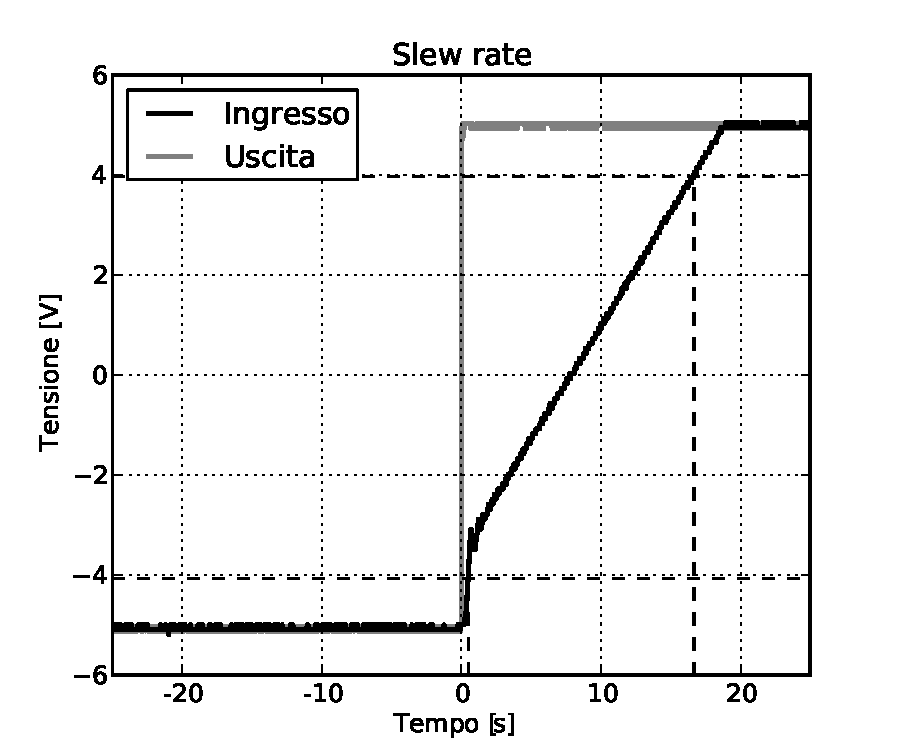
\includegraphics[width=\columnwidth]{figure/slew_graph1.pdf}
    \caption{La figura mostra il comportamento dell'operazionale ad un brusco cambiamento della tensione
        differenziale in ingresso. Il circuito realizzato (il \ref{fig:slew_circ3}) è un emitter follower
        e dovrebbe copiare il segnale in ingresso all'uscita. Invece, a causa del fatto che lo slew rate
        dell'operazionale è finito, la tensione impiega circa 20 $\mu$s a passare da -5 V a 5 V.}
    \label{fig:slew_graph3}
\end{figure}

Per la misura si fornisce in input un'onda quadra generata con il generatore
di funzioni d'onda (Che ha uno slew rate molto alto che fa si che il suo output sia
molto vicino ad un onda quadra. Abbiamo misurato uno slew rate di circa 500 V/$\mu$s per
il nostro generatore.) e si misura $V\ped{out}$, che è un trapezio a causa appunto dello
slew rate finito dell'operazionale. La figura  \ref{fig:slew_graph3} mostra un esempio
di quello che succede dando in ingresso un onda quadra.
Per convenzione, si misura il tempo impiegato
dalla tensione per salire dal 10\% al 90\% della tensione massima dello scalino.
Lo slew rate è calcolabile così:

\begin{equation}
    S = \frac{V\ped{90\%} - V\ped{10\%}}{t\ped{90\%} - t\ped{90\%}}
\end{equation}

Nelle nostre misure abbiamo utilizzato un onda quadra di 10 Vpp a 1 kHz.
Misurando lo slew rate sia in salita che in discesa, e abbiamo ottenuto
due valori diversi

\begin{equation}
    S\ped{salita} = 0.498 \pm 0.004 \; \text{V/$\mu$s}
\end{equation}
\begin{equation}
    S\ped{discesa} = -0.353 \pm 0.003 \; \text{V/$\mu$s}
\end{equation}

Il valore in salita è vicinissimo al dato specificato dal produttore: 0.5 V/$\mu$s.
Il dato in discesa è minore circa del 30\% rispetto a quello in salita.

Lo slew rate ha implicazioni piuttosto pesanti ad alte frequenze di funzionamento del circuito.
Infatti se all'amplificatore operazionale è dato in input un segnale che varia in maniera molto
veloce (un segnale periodico ad alta frequenza), ad un certo punto l'amplificatore non riuscirà
più a ''star dietro``, per così dire, al segnale, e inizierà a deformarlo. Per verificare questo
comportamento, abbiamo usato lo stesso circuito di prima, ma il generatore di forme d'onda è
stato impostato per fornire un'onda sinusoidale 10 Vpp di divese frequenze. Variando la frequenza
abbiamo notato che il segnale inizia ad essere deformato a circa 13 kHz (solo in discesa ovviamente,
poiché lo slew rate è minore). In figura \ref{fig:slew_signal3} sono mostrati input e output
alla frequenza di 20 kHz. La deformazione del segnale è evidente sia in salita che in discesa ed è
pure abbastanza seria, nonostante la frequenza non sia poi così alta (è grande l'ampiezza del segnale).

\begin{figure}
    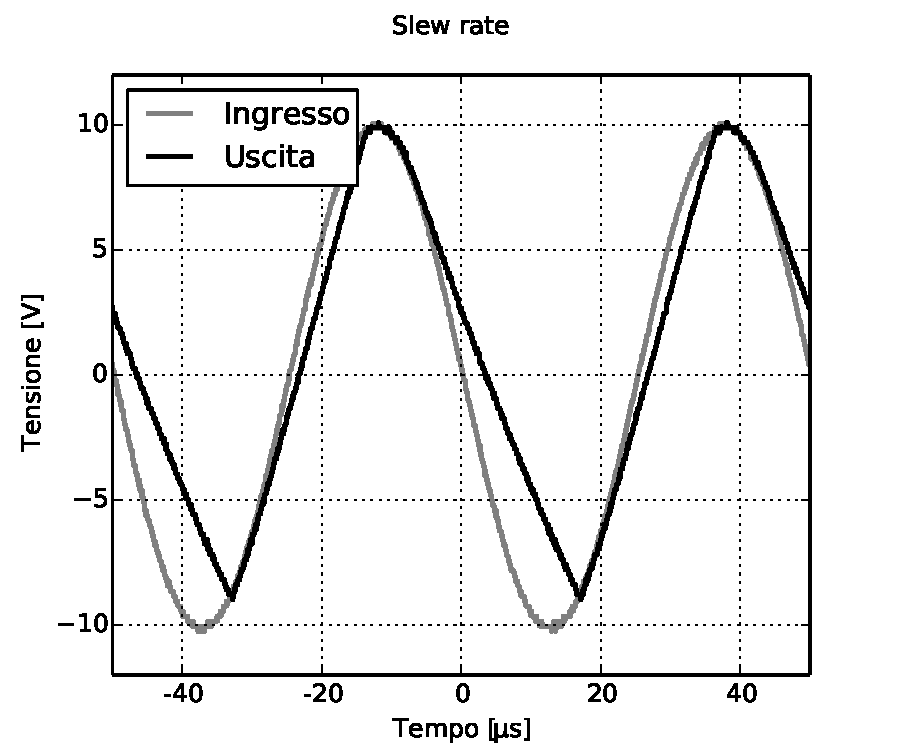
\includegraphics[width=\columnwidth]{figure/slew_signal3.pdf}
    \caption{La figura mostra il comportamento dell'operazionale ad un brusco cambiamento della tensione
        differenziale in ingresso. Il circuito realizzato (il \ref{fig:slew_circ3}) è un emitter follower
        e dovrebbe copiare il segnale in ingresso all'uscita. Invece, a causa del fatto che lo slew rate
        dell'operazionale è finito, la tensione impiega circa 20 $\mu$s a passare da -5 V a 5 V.}
    \label{fig:slew_signal3}
\end{figure}

\paragraph{Corrente massima.}

In questo paragrafo ci proponiamo di misurare la corrente massima che il nostro amplificatore
riesce a fornire dall'uscita. Per la misura ci siamo serviti del circuito \ref{fig:max_curr_circ3}.
Il circuito è semplicissimo: è simile al precedente, ma tra l'uscita e terra è presente solo una resistenza
molto piccola (100 \si{\ohm}) in modo che la tensione $v\ped{out}$ non sia determinata dalla tensione
in ingresso, bensì dalla massima corrente che l'amplificatore riesce a fornire. Misurando $V\ped{out}$.
si ricava banalmente la corrente dalla legge di Ohm, assumendo che la corrente assorbita dall'ingresso
invertente sia trascurabile.

Abbiamo fornito in input un'onda triangolare di 10 Vpp a 1 kHz. L'uscita registrata è stata un'andamento,
sempre triangolare, di 2.7 V da picco a picco. Dividendo a metà (cioè prendendo la massima tensione che $V\ped{out}$
assume, nell'altra metà dell'onda la corrente scorre semplicemente al rovescio) e usando la legge di Ohm
si ottiene $I\ped{max} = 13.5 \pm 0.7$ mA. Il range tipico riportato sul manuale è 10-20 mA.

\paragraph{Banda passante.}

\begin{figure*}[t]
    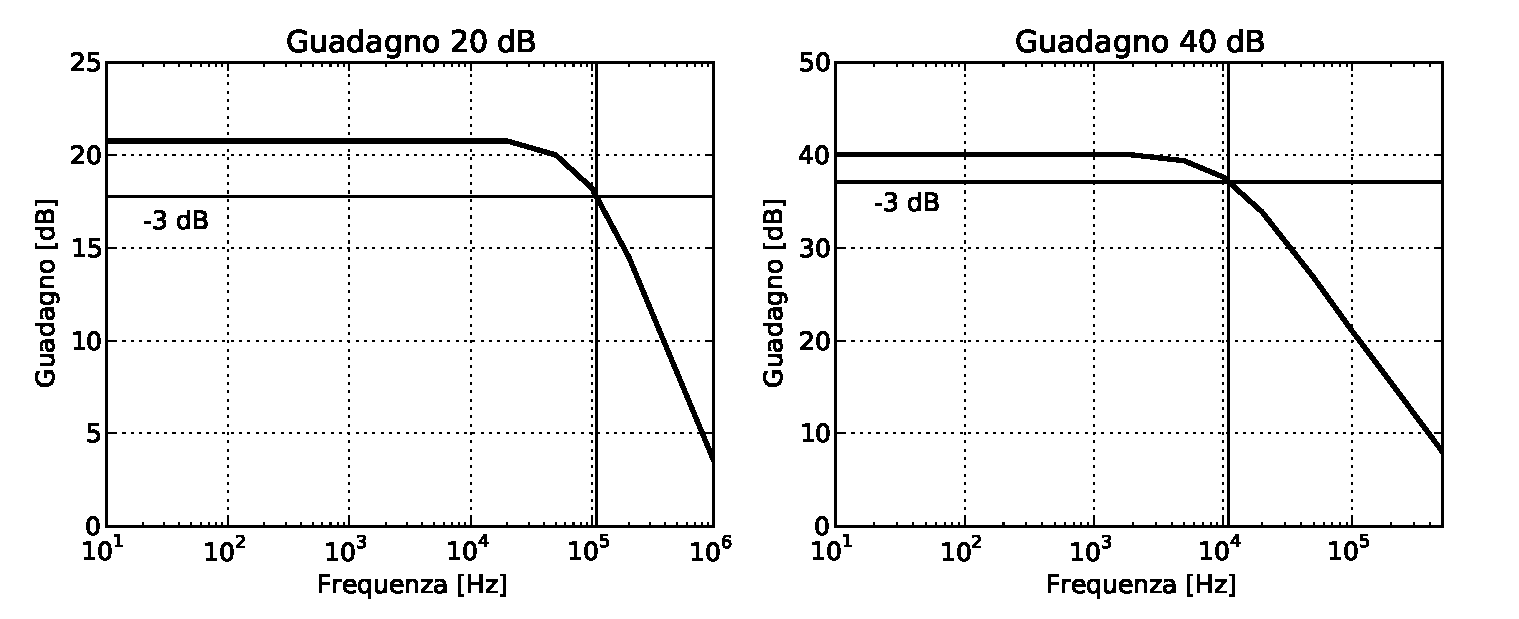
\includegraphics[width=\textwidth]{figure/freq_ris.pdf}
    \caption{La figura mostra l'amplificazione in frequenza del circuito \ref{fig:banda_circ3}
        nelle due varianti con guadagno di 20 db e 40 db circa. I circuiti si comportano come filtri
        passa basso con frequenza di taglio di $108 \pm 6$ kHz (20 db) e $11 \pm 5$ kHz (40 db).
        Sono filtri di primo ordine, con un'attenuazione di 20 db per decade.}
    \label{fig:freq_ris3}
\end{figure*}

La banda passante di un circuito è la banda di frequenze nella quale il segnale non viene attenuato.
Quantitativamente si considera l'intervallo dello spettro in frequenza del circuito tra le
frequenze alle quali il segnale viene attenuato di -3 dB rispetto al massimo, cioè le frequenze di taglio. Abbiamo quindi
registrato la risposta in frequenza del circuito \ref{fig:banda_circ3}, che è un semplice amplificatore
non invertente di guadagno $G = R_2/R_1$. Abbiamo considerato due configurazioni del circuito:
una con $R_2 = \SI{10}{\kilo\ohm}$ e l'altra con $R_2 = \SI{100}{\kilo\ohm}$, mentre $R_1 = \SI{1}{\kilo\ohm}$
in entrambi i casi. I due circuiti amplificavano quindi 20 dB e 40 dB rispettivamente.

Abbiamo quindi fornito in ingresso una sinusoide di $V = 50$ mVpp e abbiamo misurato con
l'oscilloscopio l'ampiezza dell'onda in uscita variando la frequenza all'ingresso.
Il valore di 50 mV è stato scelto perché volevamo fare misure fino a 1 MHz circa e non volevamo
che lo slew rate dell'amplificatore influisse sulle misure. Infatti a 1 MHz un onda sinusoidale
va dal massimo al minimo in 0.5 $\mu$s e quindi è necessario che l'ampiezza sia al massimo 0.25 V (assumendo 0.5 V$\mu$s)
affinché l'operazionale non abbia problemi. In realtà la pendenza massima della sinusoide è ancora maggiore,
quindi per essere conservativi abbiamo scelto 1/5 del valore massimo. Successivamente,
calcolando in ogni punto il guadagno in decibel con la formula $G = 20\log_{10}(R_2/R_1)$
e plottando i valori in funzione della frequenza, abbiamo ottenuto i grafici in figura \ref{fig:freq_ris3}.
La banda passante dei due circuiti è:

\begin{itemize}
    \item{Da zero a $108 \pm 6$ kHz per il circuito con guadagno 20 dB.}
    \item{Da zero a $11 \pm 5$ kHz per il circuito con guadagno 20 dB.}
\end{itemize}

Il fatto che il guadagno di questi circuiti non sia costante su tutte le frequenze è dovuto al fatto che ad alte frequenze
il guadagno open loop dell'operazionale diminuisce di molto e quindi la retroazione non funziona più come dovrebbe.
Con queste misure volevamo mostrare proprio questo fatto, che rappresenta l'ultimo aspetto degli amplificatori
operazionali reali che vogliamo andare a studiare. Infatti il guadagno open loop non è costante, ma fortemente dipendente
dalla frequenza, come mostreremo nel seguente paragrafo.

\paragraph{Guadagno in funzione della frequenza.}

Abbiamo sempre detto che un operazionale ha un guadagno differenziale enorme, dell'ordine di 100-120 dB
(nel caso ideale sarebbe infinito). Tuttavia questo è vero solo a frequenze molto basse, dell'ordine dei
10 Hz. A frequenze più alte il guadagno si riduce notevolmente, fino a diventare unitario attorno ad 1 MHz.

La misura del guadagno è difficile, soprattutto a basse frequenze, poiché il guadagno è enorme e la misura
diretta è impossibile. Inoltre a causa dell'enorme guadagno una misura senza retroazione è praticamente
impossibile, perché anche piccole tensioni DC in ingresso (dovute a rumore o al genratore di forme d'onda o anche la semplice
tensione di offset che è impossibile eliminare completamente)
vengono amplificate moltissimo, portanto l'output in saturazione.

La soluzione è utilizzare l'intelligente circuito \ref{fig:gain_low_circ3}. Abbiamo usato le resistenze
$R_3 = \SI{100}{\kilo\ohm}$ e $R_4 = \SI{100}{\ohm}$. Nel circuito il segnale in ingresso $V$ è simile
alla tensione presente in $V_A$. Il partitore di tensione formato da $R_3$ ed $R_4$ fa si che all'ingresso
invertente sia presente una tensione $V_A \cdot [R_3 / (R_3 + R_4)] = V_A/1001$. Il ramo di feedback serve a impedire all'operazionale di
saturare, mentre $R_1$ è necessaria al corretto funzionamento del feedback (altrimenti $V_A$ sarebbe costretta ad
essere uguale a $V$, e quindi il feedback non agirebbe). Misurando $V_A$ e $V\ped{out}$ e sapendo
che il comportamento dell'amplificatore è modellizzato dalla formula $V\ped{out} = A(V^+ - V^-)$, dove $V^+$ e $V^-$ sono
le tensioni agli ingressi non invertente ed invertente rispettivamente, mentre A è il guadagno che vogliamo
misurare, si ha:

\begin{equation}
    A = \frac{R_3 + R_4}{R_3}\frac{V\ped{out}}{V_A} = 1001\,\frac{V\ped{out}}{V_A}
\end{equation}
%
(Il segno meno è sparito perché noi consideriamo solo l'ampiezza, e non la fase, di $V\ped{out}$ e $V_A$.)

È importante notare che all'aumentare della frequenza il guadagno diminuisce e quindi, a parità
di input, $V_A$ aumenta, mentre $V\ped{out}$ diminuisce. Ad un certo punto questo andamento è controproducente
perché $V\ped{out}$ diventa troppo piccola per una misura affidabile. Al raggiungimento di questo
punto abbiamo quindi deciso di utilizzare il circuito \ref{fig:gain_high_circ3} che permette una
semplice misura diretta del guadagno, mediante la formula:

\begin{equation}
    A = \frac{V\ped{out}}{V_A}
\end{equation}

Per le misure abbiamo utilizzato la canonica onda sinusoidale di 50 mVpp (sempre per non avere
problemi con lo slew rate). Il grafico in figura \ref{fig:A_vs_freq3} mostra l'andamento misurato,
che è simile al grafico tipico riportato sul manuale. L'amplificatore ha un guadagno in continua di
99.9 $\pm$ 0.4 dB (circa la metà del valore tipico 106 dB), e si comporta come un filtro RC con un'attenuazione
di 20 dB/decade (6 db/ottava).

\begin{SCfigure*}
    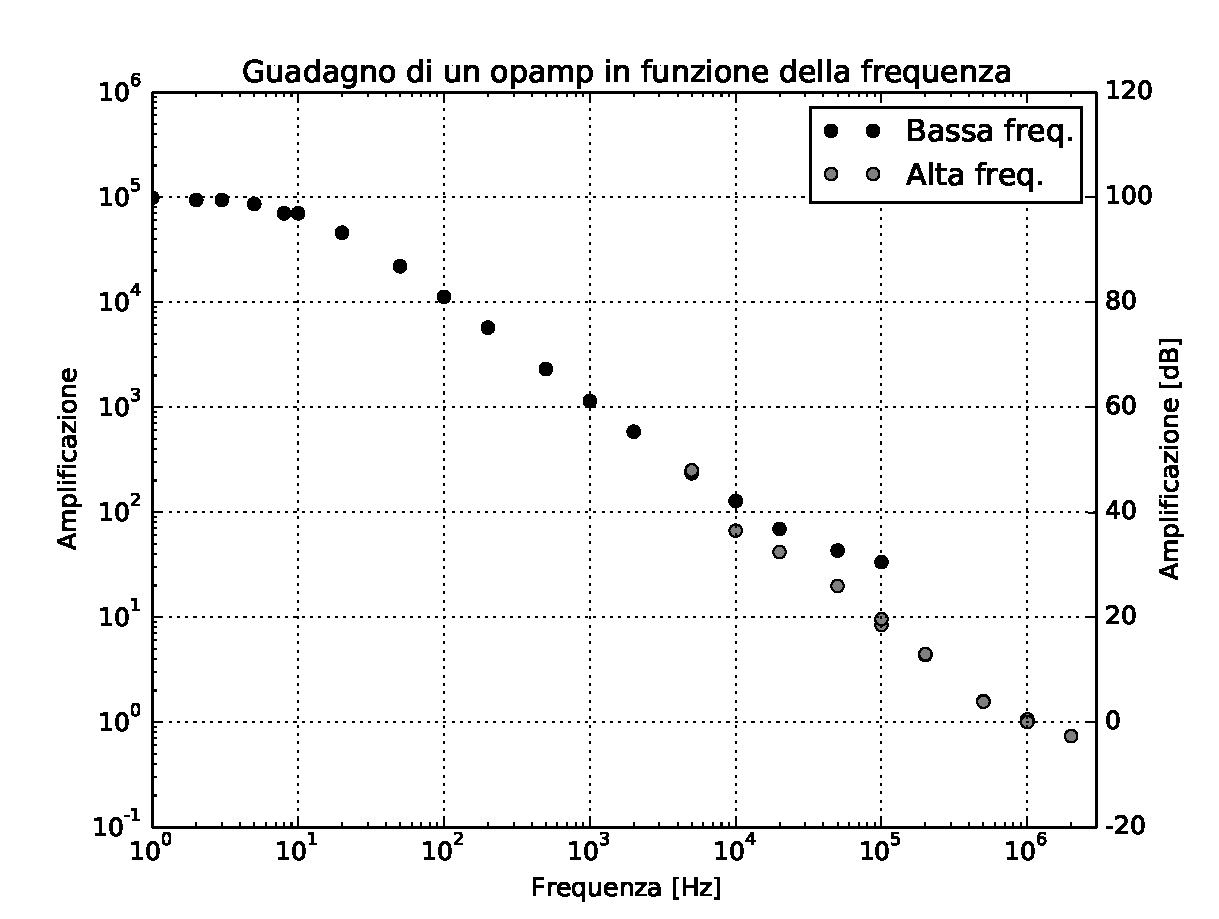
\includegraphics[width=0.7\textwidth]{figure/A_vs_freq.pdf}
    \caption{Il grafico mostra l'andamento del guadagno open loop dell'amplificatore operazionale UA741
        in funzione della frequenza. Come si vede il guadagno è massimo solo in una ristretta banda di
        frequenze, fino a circa 8 Hz. Poi il guadagno diminuisce ad un decimo ogni decade.
        I punti neri sono stati rilevati con il circuito \ref{fig:gain_low_circ3} e si vede
        che a frequenze alte l'incertezza diventa cospicua, mentre
        quelli grigi sono stati misurati con il circuito \ref{fig:gain_high_circ3}. Nei punti dove l'incertezza non
        è visibile essa è minore della dimensione dei punti. Il guadagno diventa unitario a circa 1 MHz.}
    \label{fig:A_vs_freq3}
\end{SCfigure*}

\begin{SCfigure*}
    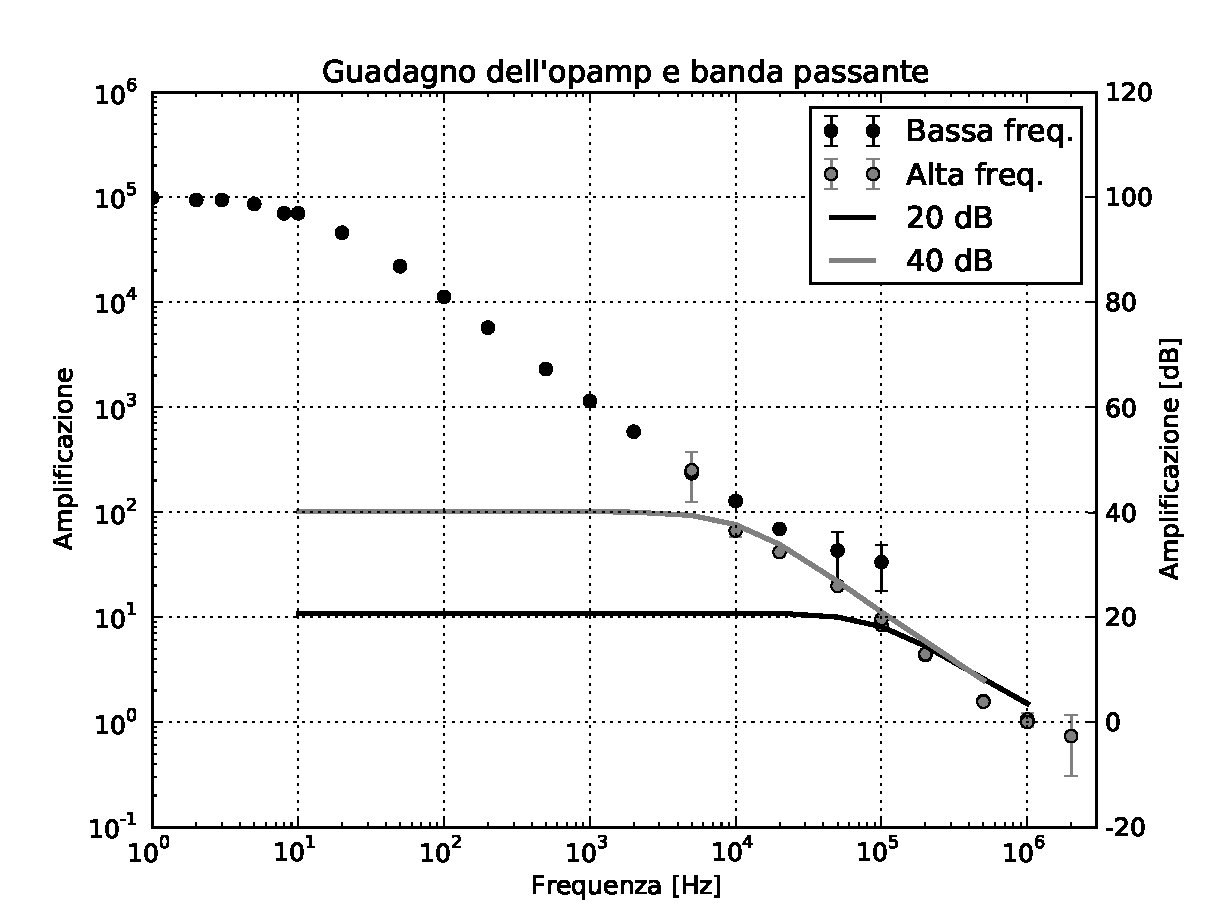
\includegraphics[width=0.7\textwidth]{figure/gabp.pdf}
    \caption{Nel grafico sono visibili gli stessi dati delle figure \ref{fig:freq_ris3} e \ref{fig:A_vs_freq3}, solo che sono
        mostrati assieme. Come si vede è proprio a causa dell'andamento del guadagno in frequenza dell'opamp che
        questi circuiti hanno una frequenza di taglio ed una riduzione del guadagno.}
    \label{fig:gabp3}
\end{SCfigure*}

Nella figura \ref{fig:gabp3} abbiamo riportato lo stesso grafico con anche gli andamenti in frequenza degli amplificatori
non invertenti del paragrafo precedente, per mostrare come l'attenuazione del segnale che si osserva in questi circuiti
sia dovuta al comportamento in frequenza dell'operazionale. Per applicazione ad alta frequenza sono disponibili
amplificatori senza condensatori all'interno.